\uuid{tIOs}
\exo7id{2849}
\titre{exo7 2849}
\auteur{burnol}
\organisation{exo7}
\datecreate{2009-12-15}
\isIndication{false}
\isCorrection{false}
\chapitre{Théorème des résidus}
\sousChapitre{Théorème des résidus}
\module{Analyse complexe}
\niveau{L3}
\difficulte{}

\contenu{
\texte{
On considère dans le plan complexe un chemin fermé paramétré
$\gamma$ qui parcourt la figure ci-dessus dans le sens indiqué. 
$$  \centerline{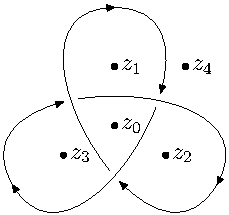
\includegraphics{../images/pdf/tIOs-1.pdf}} $$

Pour $j = 0, 1, 2, 3, 4$ on note \[A_j = \frac1{2\pi i} \int_\gamma \frac{dz}{z -z_j}\quad\text{et}\quad B_j = \frac1{2\pi i} \int_\gamma \frac{dz}{(z - z_j)^2}\] Déterminer, en le justifiant, les valeurs de $A_0$, $A_1$, $A_2$, $A_3$, $A_4$, et de $B_0$, $B_1$, $B_2$, $B_3$, $B_4$. On précisera aussi quel est le nom que l'on donne aux quantités données par les intégrales $A_j$, $j= 0\dots4$.
}
}
